\documentclass[hide notes,intlimits]{beamer}

\mode<presentation>
{
  \usetheme[footline]{UAFshade}
  \setbeamercovered{transparent}
}
% frames are 128 millimeters by 96 millimeters
% load packages
\usepackage[english]{babel}
\usepackage[latin1]{inputenc}
\usepackage[T1]{fontenc}
\usepackage{amsmath,amssymb,wasysym}
\usepackage{lmodern}
\usepackage{movie15}
\usepackage{tikz}
\usetikzlibrary{shapes,arrows}


% Some useful commands (from MPL)
\newcommand{\s}[1]{\ensuremath{\,\text{#1}}}
\newcommand{\unit}[1]{\ensuremath{\,\text{#1}}}

\definecolor{dark red}{HTML}{E41A1C}
\definecolor{dark green}{HTML}{4DAF4A}
\definecolor{dark violet}{HTML}{984EA3}
\definecolor{dark blue}{HTML}{084594}
\definecolor{dark orange}{HTML}{FF7F00}
\definecolor{light blue}{HTML}{377EB8}
\definecolor{light red}{HTML}{FB9A99}
\definecolor{light violet}{HTML}{CAB2D6}

\setbeamercolor{boxed}{fg=black,bg=uaf yellow}


\graphicspath{{figures/}}

\usetikzlibrary{shadows}

\newenvironment{transbox}{%
  \begin{tikzpicture}
    \node[drop shadow,rounded corners,text width=\textwidth,fill=white, fill opacity=0.6,text opacity=1] \bgroup
  }{
    \egroup;\end{tikzpicture}} 

\newenvironment{transbox-tight}{%
  \begin{tikzpicture}
    \node[drop shadow,rounded corners,fill=uaf yellow, fill opacity=0.75,text opacity=1] \bgroup
  }{
    \egroup;\end{tikzpicture}} 


% title page
\title[PISM (the Parallel Ice Sheet Model)] % (optional, use only with long paper titles)
{PISM (the Parallel Ice Sheet Model)}
\subtitle{Latest 0.5 release, and \\ Where will this community take PISM?}


\author[Bueler] % (optional, use only with lots of authors)
{Ed Bueler}
% - Give the names in the same order as the appear in the paper.
% - Use the \inst{?} command only if the authors have different
% affiliation.
\institute{
University of Alaska Fairbanks
}

\date{European PISM Workshop, May 2012}
%\subject{PISM: Current status and future plans}


\begin{document}

% define what is shown at the beginning of each section
\AtBeginSection[]
{
 \begin{frame}<beamer>
   \frametitle{Outline}
   \tableofcontents[currentsection,subsectionstyle=hide/hide/hide]
 \end{frame}
}


\setbeamertemplate{background canvas}
{
  \tikz{\node[inner sep=0pt,opacity=1.0] {\includegraphics[width=\paperwidth]{uaf_beamer_shade_bg}};}
} 

% insert titlepage
\begin{frame}
  \titlepage
\end{frame}

\setbeamertemplate{background canvas}
{
  % empty
}

\section[introduction]{introduction to PISM in XXX slides}

\begin{frame}
  \frametitle{PISM: new user's point of view}
  \begin{columns}
    \begin{column}{50mm}
      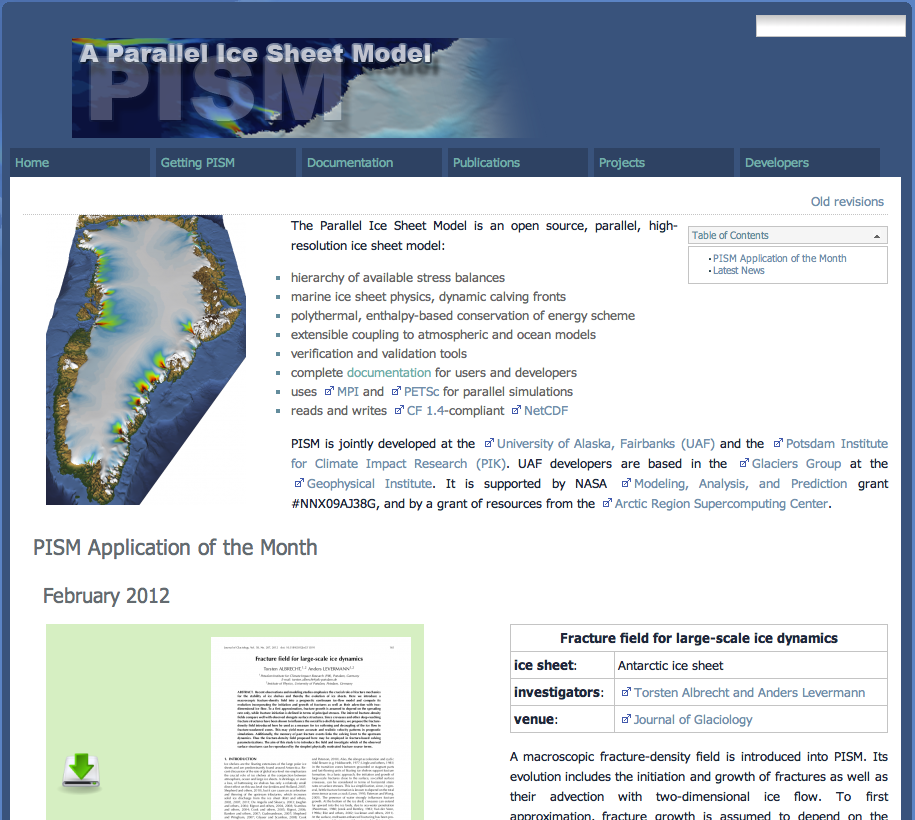
\includegraphics[width=50mm]{pismdocs.png}
    \end{column}
    \begin{column}{70mm}
      \begin{itemize}
      \item website: \alert{www.pism-docs.org}
      \item PISM runs on Linux, Unix, and Mac OSX: laptops to supercomputers
      \item stable releases once a year
      \item designed with usability in mind
      \item comprehensive User's Manual with real modeling examples
      \item \url{help@pism-docs.org}
      \end{itemize}
    \end{column}
  \end{columns}
\end{frame}


\begin{frame}
  \frametitle{PISM: power user's point of view}
  \begin{itemize}
  \item hosted at \texttt{github.com/pism/pism}
  \item modular and extensible C++ code base
  \item documented source code (\texttt{doxygen})
  \item everything is parallel (PETSc and MPI)
    \begin{itemize}
    \item whole Antarctica at 5 km resolution
    \item whole Greenland at 1 km resolution for 100 model years
      \begin{itemize}
      \item $\approx$ 100k processor-hours on 512 cores at ARSC
      \item Gollege at VUW has done bigger for New Zealand ice sheet
      \end{itemize}
    \end{itemize}
  \item open source (GPL)
  \item effective, well-tested physics
    \begin{itemize}
    \item shallow hybrid
    \item enthalpy method
   \end{itemize}
  \end{itemize}
\end{frame}


\begin{frame}
  \frametitle{who supports development?}
  \begin{itemize}
 \item supported by the NASA Modeling, Analysis and Prediction grant NNX09AJ38G
   (2009--2013)
   \item earlier NASA grant too (2003--2008)
  \item since April 2011: jointly developed by UAF and the Potsdam
    Institute for Climate Impact Research (PIK)
  \item the community of developers likely to expand in the next year!
  \end{itemize}
\end{frame}


\begin{frame}
  \frametitle{a community of users}
 \begin{center}
    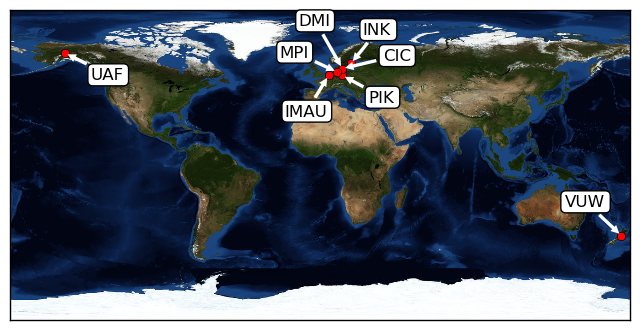
\includegraphics[width=120mm]{pism-users-map.png}
  \end{center}
\end{frame}


\begin{frame}
  \frametitle{Publications}

  \begin{itemize}
  \item in the 17 months since the start of 2011: \alert{14 papers} using PISM have been published or are ``in press''
  \item see the website:
    \begin{center}
    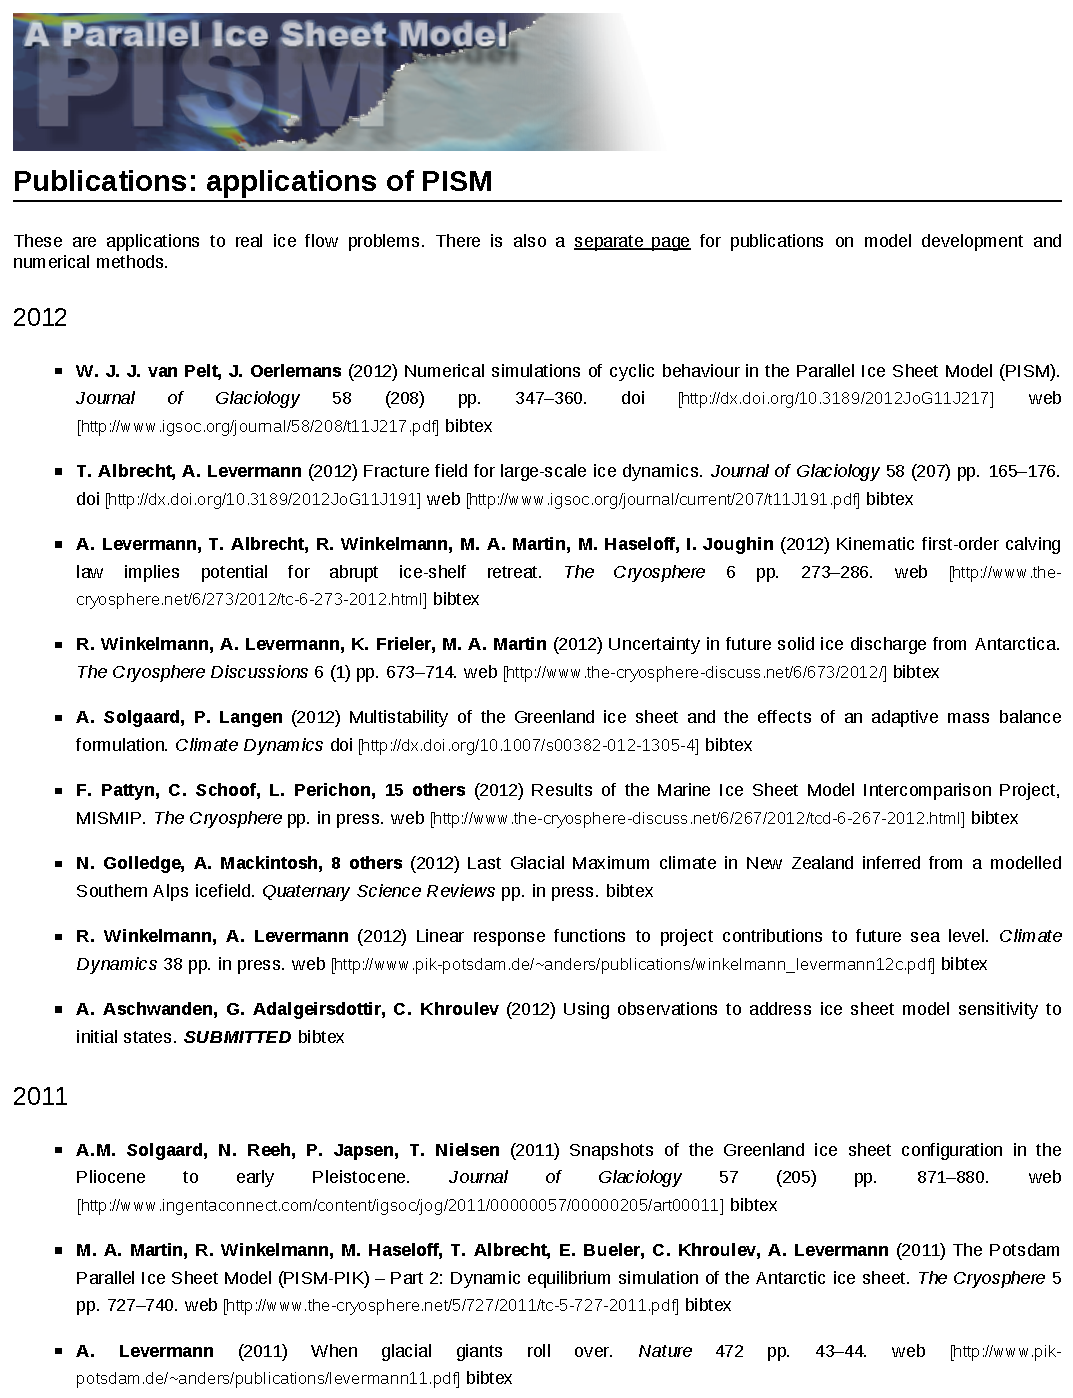
\includegraphics[height=0.65\textheight]{publications}
    \end{center}
  \end{itemize}
\end{frame}


\begin{frame}
  \frametitle{one project per month featured at website}
  \begin{center}
    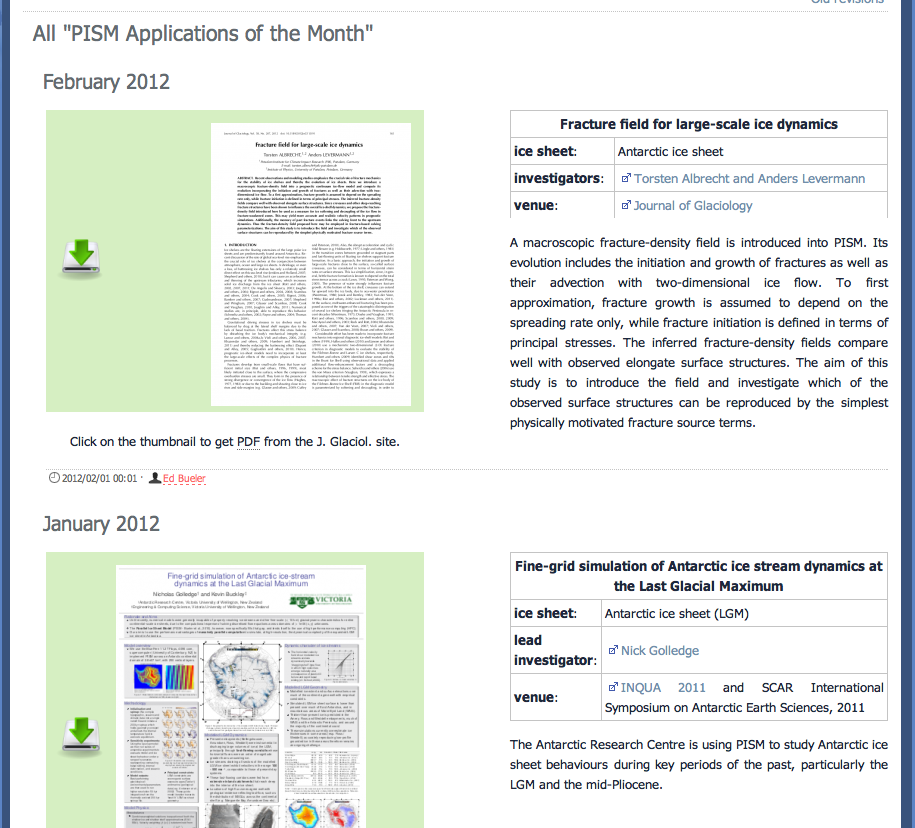
\includegraphics[height=0.75\textheight]{application-of-the-month.png}
  \end{center}
\end{frame}


\begin{frame}
  \frametitle{who answers \texttt{help@pism-docs.org}?}
  \begin{columns}
    \begin{column}{0.5\textwidth}
      \begin{center}
      %\includegraphics[width=1.0\textwidth]{}
      FIXME
      
      Constantine Khroulev
      \end{center}
    \end{column}
    \begin{column}{0.5\textwidth}
      \begin{center}
      %\includegraphics[width=1.0\textwidth]{}
      FIXME
      
      Andy Aschwanden
      \end{center}
    \end{column}
  \end{columns}

\end{frame}


\begin{frame}
  \frametitle{minimal history}
  \begin{itemize}
  \item 1984--2001: Craig Lingle does lonely ice sheet/stream modeling
  \item 2002--2004:
    \begin{itemize}
    \item[$\circ$] Craig recruits Jed Brown and me as developers
    \item[$\circ$] Jed decides on PETSc
    \end{itemize}
  \item 2005: first draft is ``COMMVNISM''
  \item 2006: first PISM release on \texttt{gna.org}
  \item 2008:
    \begin{itemize}
    \item[$\circ$] Constantine
    \item[$\circ$] PIK visits Alaska
    \end{itemize}
  \item 2009: Andy
  \item 2011:
    \begin{itemize}
    \item[$\circ$] merge PISM-PIK
    \item[$\circ$] move to \texttt{github.com}
    \end{itemize}
  \end{itemize}
\end{frame}


\section[latest release]{latest release  (XXX slides)}

\begin{frame}
  \frametitle{\texttt{stable0.5} release June 2012}

  \begin{itemize}
  \item get pre-release now:
    \begin{center}
    \texttt{git clone git://github.com/pism/pism.git pism0.5}
    \end{center}
  \item June ``official'' release after more testing, documentation
    \begin{itemize}
    \item[$\circ$] watch for CYROLIST announcement
    \item[$\circ$] then do ``\texttt{git pull}'' and recompile then
    \end{itemize}
  \item changes improve usability\!
  \item changelog from 0.4:
    \begin{itemize}
    \item[$\circ$] requires PETSc 3.2
    \item[$\circ$] \texttt{-o\_format [netcdf4\_parallel, pnetcdf]}
    \item[$\circ$] improved documentation of climate forcing code
    \item[$\circ$] many other ``evolutionary'' not ``revolutionary'' changes \dots
    \end{itemize}
  \end{itemize}
\end{frame}


\begin{frame}
  \frametitle{NetCDF4 means bigger scales}

  \begin{itemize}
  \item one limitation on fine grids was ability to write large model results fast
  \item use of parallel NetCDF4 (or \texttt{pnetcdf} also) allows it
  \item can do 1km Greenland runs for 100 model years:
    \begin{center}
    FIXME %\includegraphics[height=0.65\textheight]{}
    \end{center}
  \end{itemize}
\end{frame}


\section[to improve]{what we know we need to improve}


\section[where to?]{where is PISM going?  (where will you lead it?)}


\begin{frame}
  \frametitle{PISM-PIK merge}
  \framesubtitle{Subgrid-scale motion of the calving front}
  \begin{columns}
    \begin{column}{60mm}
      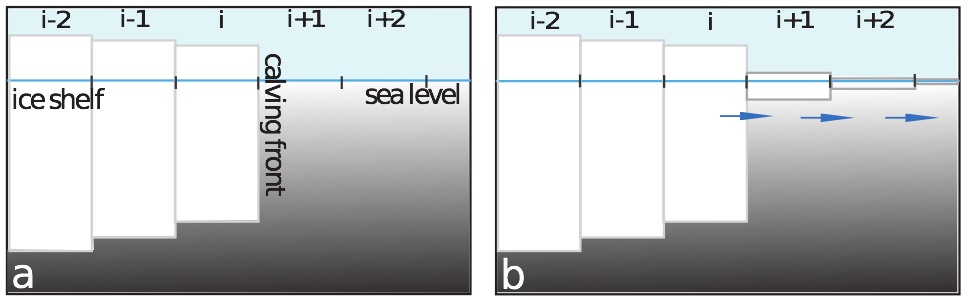
\includegraphics[width=60mm]{part-grid-scheme-1.png}\\
      \rule{0pt}{5mm}\\
      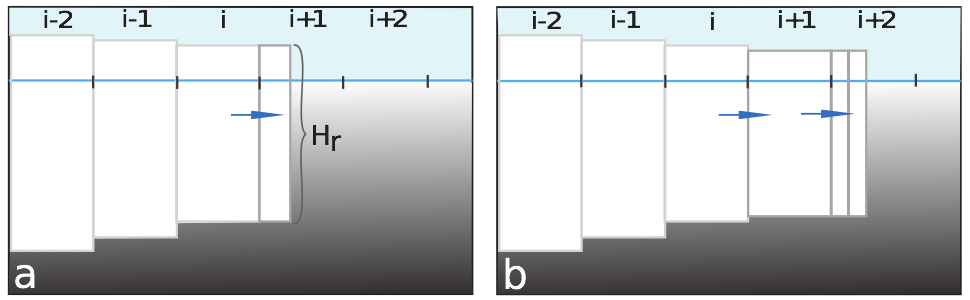
\includegraphics[width=60mm]{part-grid-scheme-2.png}\\
   \end{column}
    \begin{column}{60mm}
      \begin{itemize}
      \item avoids artificial thinning
      \item better modeling of the location of the front
      \item allows for advancing shelves
      \end{itemize}
   \end{column}
  \end{columns}
   \begin{flushleft}
      \tiny \textbf{Albrecht et al} (2011)
      \emph{Parameterization for subgrid-scale motion of ice-shelf calving
        fronts}. The Cryosphere 5 pp. 35--44.
   \end{flushleft}
\end{frame}

\begin{frame}
  \frametitle{PISM-PIK merge}
  \framesubtitle{First-order calving law}
  \begin{columns}
    \begin{column}{50mm}
      \begin{center}
        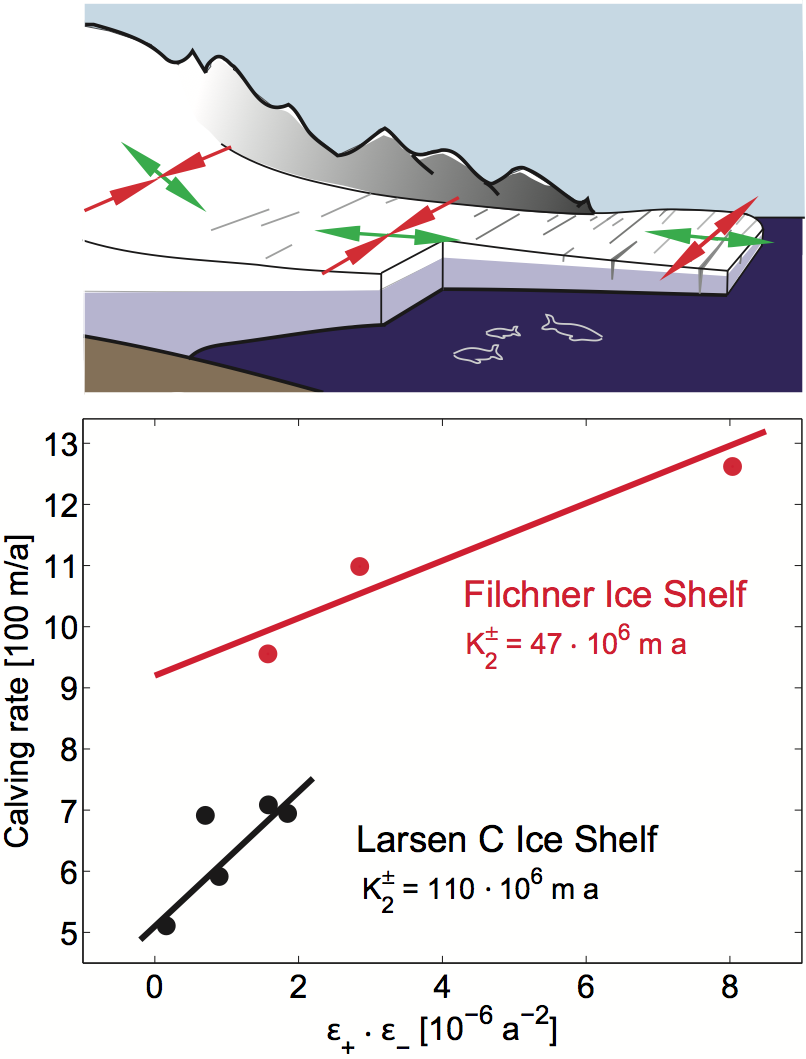
\includegraphics[height=0.6\textheight]{calving-law.png}
      \end{center}
    \end{column}
    \begin{column}{70mm}
      \begin{itemize}
      \item calving rate proportional to spreading rates in both
        eigen-directions:
        $$C = K_{2}^{\pm} \cdot \dot \epsilon_{+} \cdot \dot \epsilon_{-}$$
      \item has one scalar parameter
      \item allows for ice shelf retreat
      \end{itemize}
    \end{column}
  \end{columns}
  \begin{flushleft}
    \tiny \textbf{Levermann et al} (2011) \emph{Kinematic
      first-order calving law implies potential for abrupt ice-shelf
      retreat}. The Cryosphere Discussions 5 (5) pp. 2699--2722.
 \end{flushleft}
\end{frame}

\begin{frame}
  \frametitle{PIK application}
  \framesubtitle{Dynamic equilibrium simulation of the Antarctic ice sheet}

  \begin{center}
    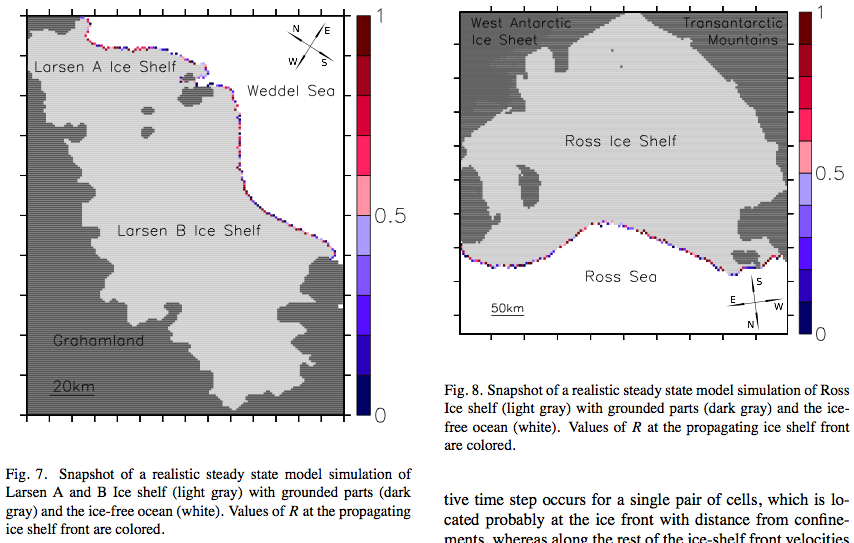
\includegraphics[height=0.7\textheight]{moving-calving-front.png}
  \end{center}
  \begin{flushleft}
    \tiny \textbf{Martin et al} (2011) \emph{The
        Potsdam Parallel Ice Sheet Model (PISM-PIK) Part 2: Dynamic
        equilibrium simulation of the Antarctic ice sheet}. The Cryosphere 5
      pp. 727--740.
  \end{flushleft}
\end{frame}

\begin{frame}
  \frametitle{PIK project}
  \framesubtitle{Fracture field for large-scale ice dynamics}
  \begin{center}
    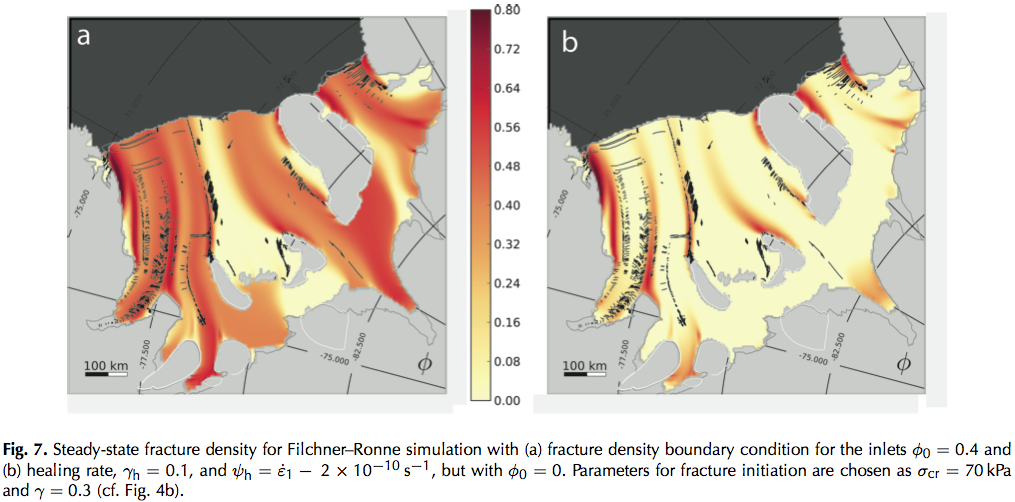
\includegraphics[width=0.9\textwidth]{fracture-density.png}
  \end{center}

  \begin{center}
    step toward fracture-based calving
  \end{center}

  \begin{flushleft}
    \tiny \textbf{Albrecht et al} (2012) \emph{Fracture field for
      large-scale ice dynamics}. Journal of Glaciology 58 (207) pp. 165--176.
 \end{flushleft}
\end{frame}

\begin{frame}
  \frametitle{UAF project}
  \framesubtitle{Enthalpy model}

  \begin{center}
    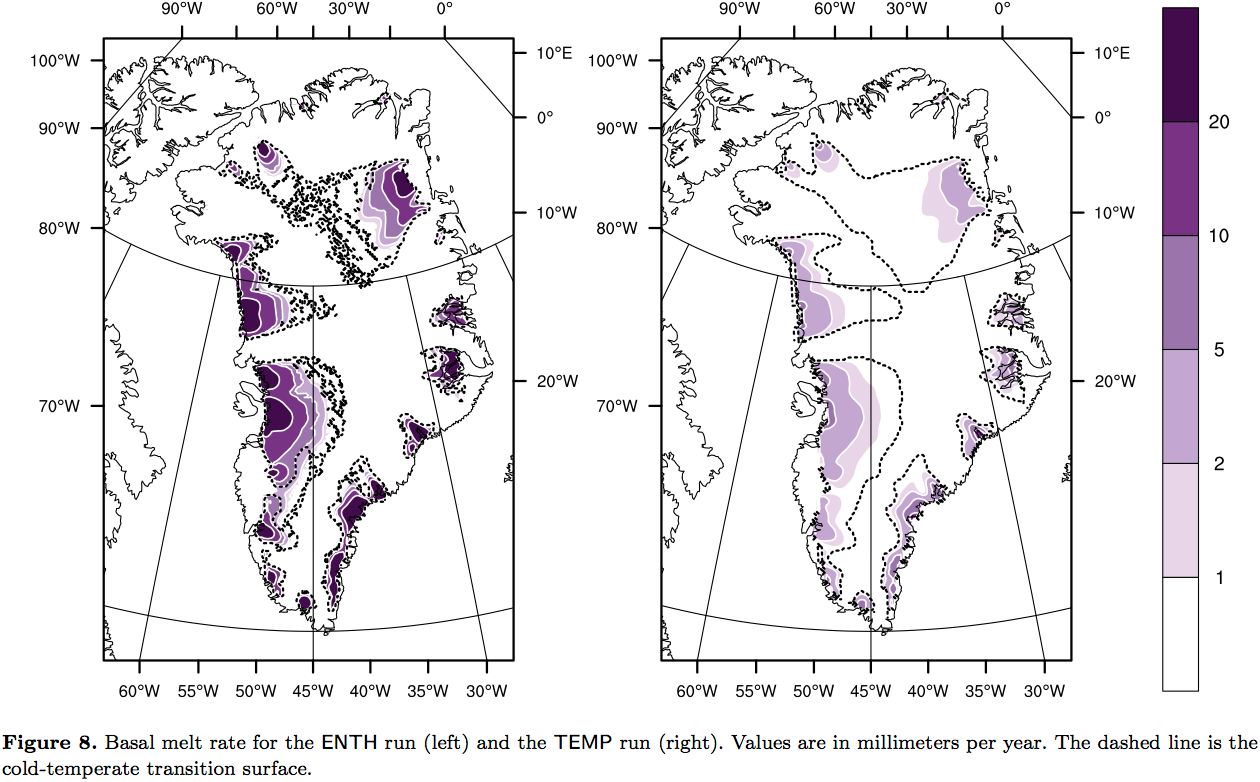
\includegraphics[height=0.7\textheight]{enthalpy-model.png}
  \end{center}

  \begin{flushleft}
  \tiny \textbf{Aschwanden et al} (2012) \emph{An enthalpy
      formulation for glaciers and ice sheets}. Journal of Glaciology, to
    appear
 \end{flushleft}
\end{frame}

\begin{frame}
  \frametitle{UAF project}
  \framesubtitle{PISM as a regional model}
  \begin{center}
    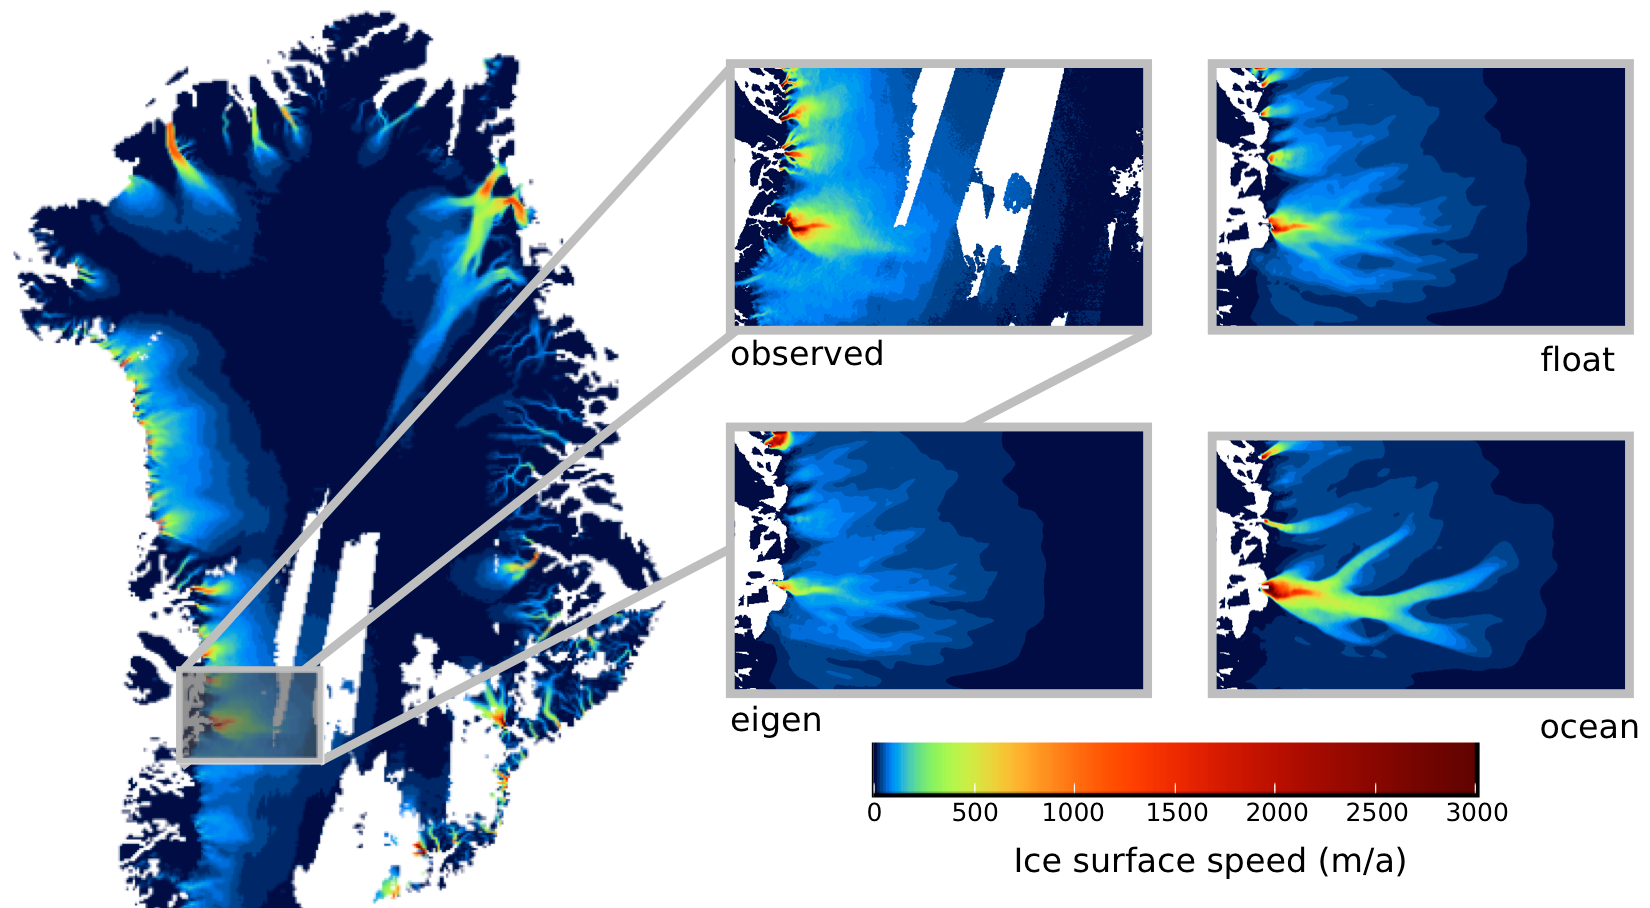
\includegraphics[width=0.95\textwidth]{csurf-regional.png}
  \end{center}
  \begin{flushleft}
    \tiny \textbf{Daniella DellaGiustina} (2011), \emph{Regional modeling of
      Greenland's outlet glaciers with the Parallel Ice Sheet Model}, M.S.
    Computational Physics thesis, UAF
  \end{flushleft}
\end{frame}

\begin{frame}
  \frametitle{UAF project}
  \framesubtitle{Validation using InSAR surface speed}
  \begin{columns}
    \begin{column}{90mm}
    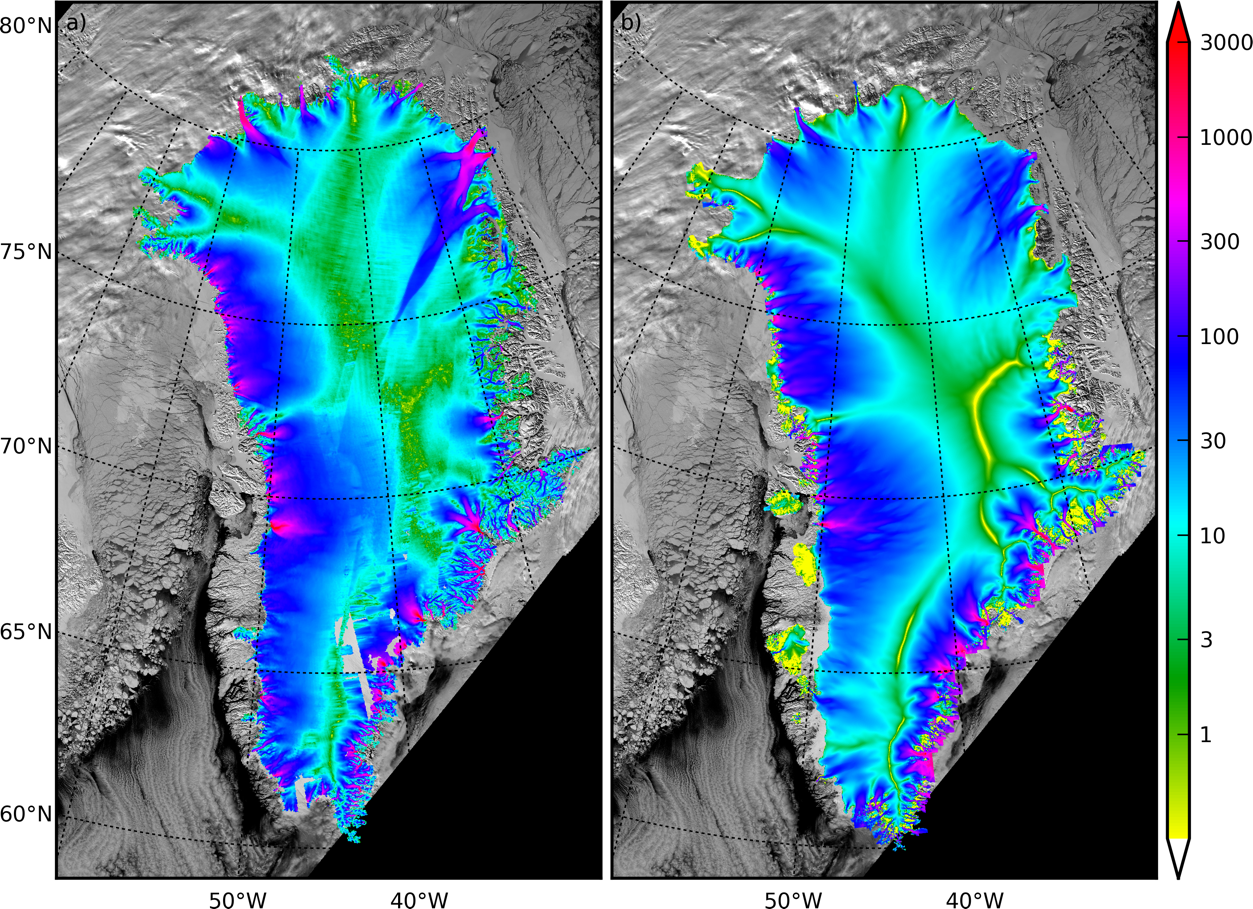
\includegraphics[width=90mm]{csurf-insar-pism-hhcmb.png}
    \begin{center}
       \tiny \textbf{Left:} InSAR surface speed in meters per year (Joughin, 2010)\\
        \textbf{Right:} PISM simulated surface speed
   \end{center}
   \end{column}

    \begin{column}{35mm}
      \begin{itemize}
      \item no inversion
      \item small number of parameters
      \item constant climate spin-up
      \item 2km grid
      \item Aschwanden et al, in prep.
      \end{itemize}
    \end{column}
  \end{columns}

\end{frame}


\begin{frame}
  \frametitle{Future plans}
  \begin{itemize}
  \item inverse modeling (lead by David Maxwell and Marijke Habermann)
    \begin{itemize}
    \item uses new tools (written in Python)
    \item shares code with PISM
    \item well under way
    \end{itemize}
  \item basal hydrology model (Ed Bueler and Ward van Pelt)
  \item Blatter stress balance solver$^{*}$
  \item better coupling
  \item better transport/advection algorithm
  \end{itemize}

 \begin{flushleft}
   \tiny
    $^{*}$ See \textbf{Brown et al} (2011)
    \emph{Achieving textbook multigrid efficiency for hydrostatic ice sheet
      flow}, submitted to SIAM J. Scientific Computing.
  \end{flushleft}
\end{frame}


\end{document}
